\section{Implementation}
In diesem Kapitel beschäftigen wir uns mit der Implementation und mit dem Aufbau von Grafana, sodass wir \gls{Cyberangriff} nach dem \gls{mitre} Matrix erkennen können. Wir gestalten unser Arbeitslabor mit \gls{container} und \glsfirst{vm}, wie in dem folgenden Diagramm dargestellt:

\begin{figure}[H]
   \centering
   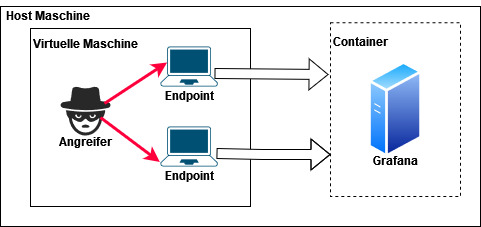
\includegraphics[width=0.5\textwidth]{assets/Arbeitslabor.jpg}
   \caption{Aufbau unseres Arbeitslabors \\Quelle: Eigene Quelle}
   \centering
\end{figure}

Von unserem Aufbau wollen wir folgende Ziele erreichen: Aufnahmen und Anpassung der Logdateien für Grafana, Musterkerennung für die ausgewählten \glsplural{Cyberangriff} und schließlich Warnmeldung für die Endnutzer, damit sie geeignete Sicherheitsmaßnahmen ergreifen können. 

Der gezielte Ablauf ist in dem folgenden Diagramm dargestellt:

\begin{figure}[H]
   \centering
   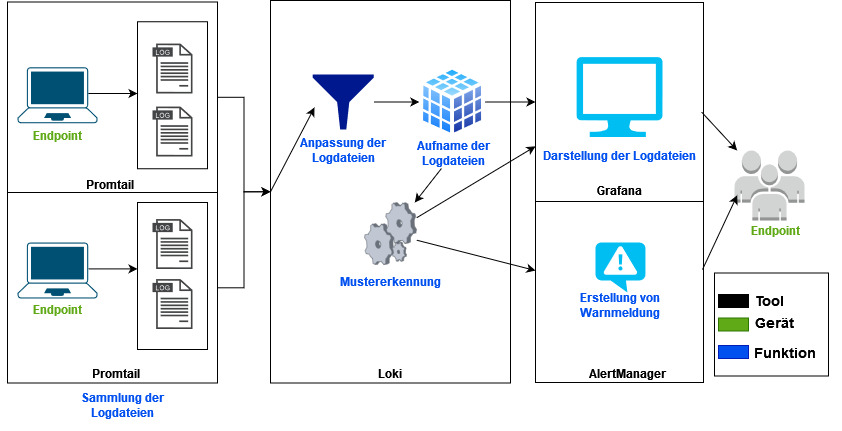
\includegraphics[width=0.7\textwidth]{assets/Ablauf_grafana2.jpg}
   \caption{Erwarteter Ablauf der Sammlung der Logdateien bis zur Warnmeldung \\ Quelle: Eigene Quelle und \citep{Grafana_loki}}
   \centering
\end{figure}

\subsection{Angriffserkennung anhand der Mitre ATT\&CK Matrix\textregistered}
Es gibt verschiedene Methoden und Frameworks zur Vermeidung, Erkennung und Unterbrechung von \glsplural{Cyberangriff}. \glsfirst{owasp}, \glsfirst{CKC} und die \gls{mitre} Matrix sind einige Beispiele, die von \gls{SOC}-Teams verwendet werden, um die Sicherheit von Systemen und/oder Netzwerken zu gewährleisten. Da sich die Richtlinien und Schwerpunkte dieser Frameworks unterscheiden können und deshalb einen anderen Aufbau unserer Struktur erfordern könnten, haben wir uns für die Anwendung der \gls{mitre} Matrix zur Erkennung von \glsplural{Cyberangriff} entschieden, insbesondere weil dieser Framework auch in Splunk integriert ist.

Die \gls{mitre} Matrix hat folgende Hauptnutzung \citep{Mitre_Started}:

{\setstretch{1.5}
\begin{itemize}[noitemsep]
   \item Erkennung und Analyse von Angriffstechnik
   \item	strukturierte Datensammlung über Bedrohungen
   \item	Emulieren von \glsplural{Cyberangriff} für die Anwendung an Angriffsübungen
   \item	Systemhärtung und Verbesserung der Verteidigungsmaßnahmen
\end{itemize}
}

Die Matrix bietet eine umfangreiche Verwendung für Unternehmen und für \gls{SOC}-Team an, um ihre wertvollen Ressource schützen und ihre Fachkenntnisse über \gls{Cybersicherheit} zu erweitern \citep{Hazel_howtousemitre}. Hier konzentrieren wir uns auf die Entwicklung und auf die Implementierung einer Methode für die automatische Erkennung und Analyse von AngriffsTechnik in Grafana.

\newpage
Die \gls{mitre} Framework besteht aus 14 Taktik. Zu jedem Taktik gehören Technik, die ihrerseits in SubTechniks aufgeteilt sind. Jede SubTechnik wird mit Beispielen, Härtungsmaßnahmen und Erkennungsregeln dargestellt.

\begin{figure}[H]
   \centering
   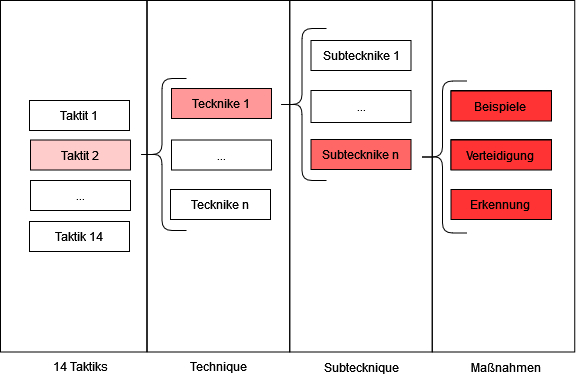
\includegraphics[width=0.8\textwidth]{assets/Mitre_structure.drawio.png}
   \caption{Struktur der Mitre Matrix \\Quelle: Eigene Quelle und \citep{Mitre_Started}}
   \centering
\end{figure}

{\setstretch{1}
Die 14 Taktiks sind folgende:
\begin{itemize}[noitemsep]
   \item Informationssammlung für zukünftige Angriffe 
   \item	Entwicklung von Ressource von Angreifer
   \item Erster Zugang zum Opfersysteme 
   \item Ausführung von bösartigen Coden
   \item Beharrlichkeit von System
   \item	Privilegienausweitung
   \item Vermeidung von Verteidigungssysteme
   \item \textbf{Zugang zu Anmeldedaten}
   \item Umgebungserkennung
   \item Seitliche Bewegung zu anderem Systemen innerhalb des Angriffsziels
   \item interne Informationssammlung
   \item Steuerung und Kontrolle (C2 - Command and Control im Original)
   \item Datenextrahierung 
   \item	Auswirkung auf die Integrität
\end{itemize}
}

\subsection{Auswahl des Angriffes}
In dieser Arbeit beschäftigen wir uns mit dem Taktik \quotes{Zugang zu Anmeldedaten} und deren Technik \gls{bruteforce}. Diese Technik ist in vier SubTechnik aufteilt:

{\setstretch{1}
\begin{itemize}[noitemsep]
   \item Erraten von Anmeldedaten 
   \item	Entschlüsselung von \glsplural{hash}
   \item \textit{\gls{stuffing}}
   \item \textit{\gls{spraying}}
\end{itemize}
}

Da unser Ziel hier ist Grafana, zu benutzen, um Angriffe zu erkennen, entschieden wir uns für einen einfachen reproduzierbaren Angriff, die weniger Ressource verlangt. In diesem Fall, lässt sich \gls{bruteforce} einwandfrei mit zwei \glsplural{vm} darstellen. Für diesen Angriff benutzen wir die SubTechnik \quotes{Erraten von Anmeldedaten und \textit{\gls{stuffing}}}, da sie ähnliche Erkennungmethode haben. Hier schließen wir auch die anderen Maßnahmen aus.

Die nächste Abbildung zeigt den Umfang unseres Implementationsversuchs:
\begin{figure}[H]
   \centering
   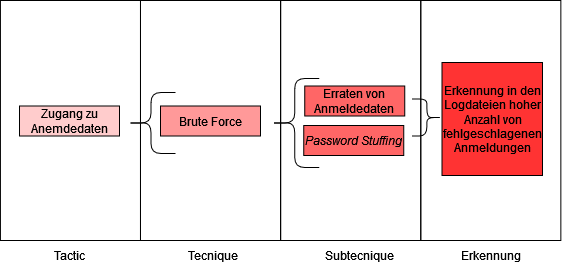
\includegraphics[width=0.8\textwidth]{assets/T1110.drawio.png}
   \caption{Analysestruktur für diese Arbeit \glsplural{Cyberangriff} \\Quelle: Eigene Quelle und \citep{Mitre_t1110}}
   \centering
\end{figure}

\newpage
\subsection{Installation und Erstellung von Logdateien}
In diesem Abschnitt fokussieren wir uns auf folgenden Punkten:

{\setstretch{1}
\begin{enumerate}[noitemsep]
   \item	Einrichtung der \glsplural{vm} für Opfersystem und Angreifen
   \item	Angriffsssimulation für die für die Generierung von Logdateien
   \item Installation und Einrichtung von Grafana Loki und Promtail mit \gls{container}
   \item Weiterleitung der Logdateien zum Grafana
\end{enumerate}
}

Die Installation und Anwendung können entweder mit dem \glsfirst{GUI} oder mit der Kommandozeilen durchgeführt werden. In dieser Arbeit benutzen wir die Kommandozeile. 

\subsubsection{Einrichtung der \glsplural{vm} für Opfersystem und Angreifen}
Die beiden \glsplural{vm} sind eine vorgebaute \quotes{\gls{kali} \glsfirst{vm}} und \quotes{\gls{ubuntu} Server 22.04.2} in ihren standardmäßigen Einstellungen. Beiden Maschinen wurden nach der jeweiligen Dokumentation installiert \citep{kali_vm} und \citep{Ubuntu_server}.

Für das Opfersystemen entschieden wir uns für die Passwörte \quotes{qwertz} und \quotes{password}. Laut einer Umfrage gehört dieses Passwort zu den zehn meisten verwendeten Passwort in Deutschland \citep{silicon_passwort}.  

Für die Durchführung von \gls{spraying} erstellen wir folgende Benutzer und Passwörterkombinationen:

{\setstretch{1.0}
\begin{Verbatim}[frame=single]
   Opfersystem 1          Opfersystem 2  
   admin:123456           bob:hallo
   user1:passwort         master:alice
   user2:abc123           hans:daniel
   user3:qwertyuiop       bruno:super123
\end{Verbatim}
}

\newpage
\subsubsection{Generierung von Logdateien mit der Angrifsssimulation}
Für den Angriff verwenden wir folgenden Tools:

{\setstretch{1.0}
\begin{itemize}[noitemsep]
   \item	\glsfirst{ssh}
   \item \gls{hydra}
\end{itemize}
}

In diesem Szenario schickt \gls{hydra} gleichzeitig mehrere Authentifizierungsversuche zum Opfersystem, um eine \gls{ssh}-Verbindung mit dem Opfersystem herzustellen. Das Tool verwendet ein sogenanntes Wörterbuch mit verschiedenen Einträgen, die als Passwörter dienen. Für unseren Test benutzen wir die bekannte \gls{rockyou}-Datei.

Die nächste Abbildung zeigt, wie \gls{stuffing} abläuft:

\begin{figure}[H]
   \centering
   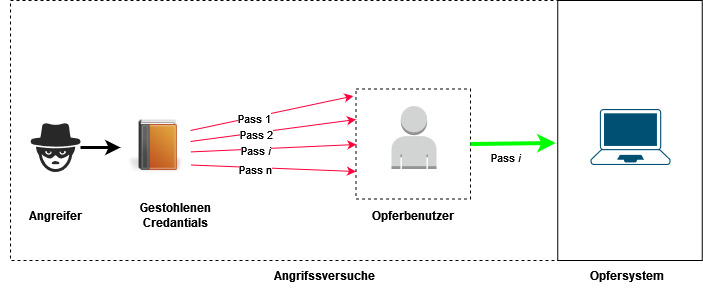
\includegraphics[width=1\textwidth]{assets/Stuffing.jpg}
   \caption{\textit{\gls{stuffing}}\\Quelle: Eigene Quelle und \citep{Nguyen_stuffing}}
   \centering
\end{figure}

\gls{stuffing} wurde mit folgendem Kommando durchgeführt \citep{kali_hydra}:
%Verbatim
{\setstretch{1.0}
\begin{Verbatim}[frame=single]
   hydra -l [Benutzername] -P rockyou.txt [Opfersystem] ssh -V -t 4

   # Erklärung
   -l: Spefizikation der Benutzername, den wir Angreifen
   -P: Auswahl der Datei mit bekannten Passwörter
   ssh: Auswahl der Anwendung, die wir angreifen wollen
   -V: Ausführliche Ausgabe über Versuche, Fehler und Erfolg
   -t 4: Anzahl von gleichzeitigen Verbindungen
\end{Verbatim}
}

Das folgende Bild zeigt ein Teil der Ausgabe von \gls{hydra} bei der Ausführung von \gls{stuffing} gegen das Opfersystem1:
\begin{figure}[H]
   \centering
   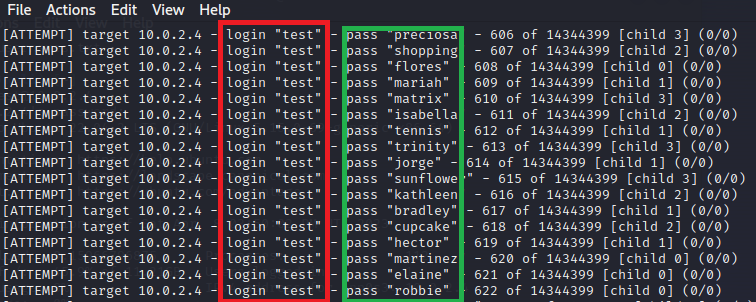
\includegraphics[width=1\textwidth]{assets/stuffing_kali.png}
   \caption{\textit{\gls{stuffing}} gegen Opfersystem1\\Quelle: Eigene Quelle und \citep{Nguyen_stuffing}}
   \centering
\end{figure}

Und gegen Opfersystem2:
\begin{figure}[H]
   \centering
   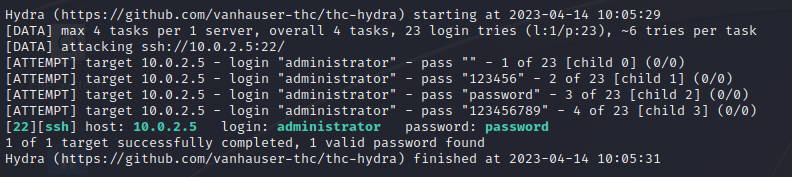
\includegraphics[width=1\textwidth]{assets/stuffing_kali2.png}
   \caption{\textit{\gls{stuffing}} gegen Opfersystem2\\Quelle: Eigene Quelle und \citep{Nguyen_stuffing}}
   \centering
\end{figure}

\newpage
Unser nächster Angriff, \gls{spraying}, sieht wie folgende aus:
\begin{figure}[H]
   \centering
   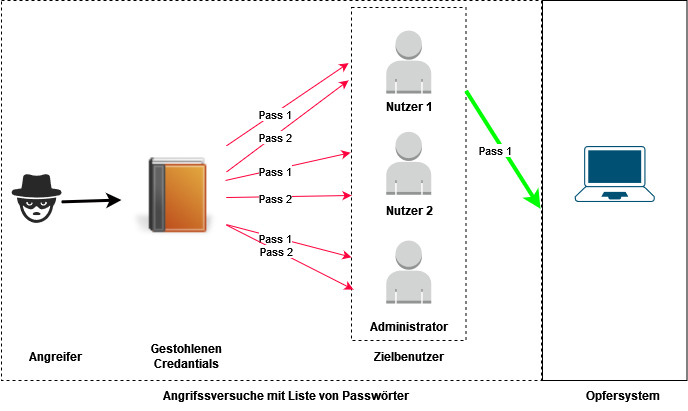
\includegraphics[width=1\textwidth]{assets/Spraying.jpg}
   \caption{\textit{\gls{spraying}}\\Quelle: Eigene Quelle und \citep{Swathi_spraxy}}
   \centering
\end{figure}

Für diesen Angriff benutzen wir folgendes Kommando:
{\setstretch{1.0}
\begin{Verbatim}[frame=single]
   hydra -L username2.txt -P passwoerter.txt [Opfersystem2] ssh -V -t 4

   # Erklärung
   -L: Auswahl der Datei mit gefunden Benutzername
\end{Verbatim}
}

In diesem Fall gehen wir davon aus, dass der Angreifer einige oder alle Benutzernamen schon kennen. Da es bei diesem Angriffe weniger Anmeldeversuche pro Nutzer stattfindet, benutzen wir eine selbsterstellte Datei mit weniger Passwörter als bei der \gls{rockyou}-Datei. Unsere Datei beinhalt die beliebigste Passwörter in Deutschland \citep{silicon_passwort}.  

\newpage
Die folgenden Screenshots zeigen die Ausführung von \gls{spraying}:
\begin{figure}[H]
   \centering
   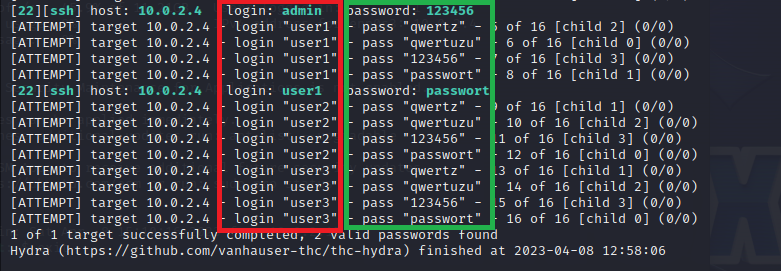
\includegraphics[width=1\textwidth]{assets/Spraying_Kali.png}
   \caption{Ausführung \textit{\gls{spraying}} in Kali Linux gegen Opfersystem1\\Quelle: Eigene Quelle}
   \centering
\end{figure}

\begin{figure}[H]
   \centering
   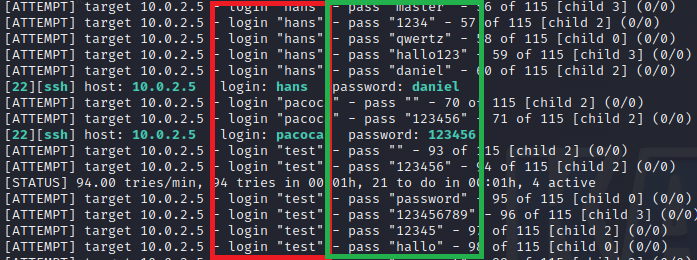
\includegraphics[width=1\textwidth]{assets/Spraying_Kali2.png}
   \caption{Ausführung \textit{\gls{spraying}} in Kali Linux gegen Opfersystem2\\Quelle: Eigene Quelle}
   \centering
\end{figure}

\newpage
\subsubsection{Installation und Einrichtung von Grafana Loki und Promtail mit \gls{container}}
Die offizielle Dokumentation von Grafana war nicht immer über die Ausführung eindeutig, deshalb benutzten wir auch fremde Quellen, um die Einstellungen an unsere Umgebung anzupassen \citep{Polinowski_PGL}. Unter befindet es sich die von Grafana zur Verfügung gestellte Konfigurationsdateien und Installationsverfahren \citep{GrafanaLoki_run}. 

{\setstretch{1.0}
\begin{Verbatim}[frame=single]
wget https://raw.githubusercontent.com/grafana/loki/v2.8.0/cmd/loki
/loki-local-config.yaml -O loki-config.yaml (die Datei wurde angepasst)

wget https://raw.githubusercontent.com/grafana/loki/v2.8.0/clients/
cmd/promtail/promtail-docker-config.yaml -O promtail-config.yaml 
(die Datei wurde angepasst)

docker-compose -f docker-compose.yaml up 
\end{Verbatim}
}
%docker run -d --name=grafana -p 3000:3000 grafana/grafana-enterprise
%docker run --name loki -d -v $(pwd):/mnt/config -p 3100:3100 grafana/loki:2.8.0 -config.file=/mnt/config/loki-config.yaml

%docker run --name promtail -d -v $(pwd):/mnt/config -v /var/log:/var/log --link loki grafana/promtail:2.8.0 -config.file=/mnt/config/promtail-config.yaml

Im Anhang befinden sich die originalle (Siehe \ref{appendix:orgGrafana}) und die angepassten Dateien (Siehe \ref{appendix:AngepasstGrafana}).

Die obigen Kommandos haben folgende Bedeutungen:
\begin{enumerate}[noitemsep]
   %\item Ausführung von Grafana und Nutzung des Nutzung des lokalen und externen \glsplural{port} 3000
   \item Herunterladen der Konfigurationsdatei von Loki
   %\item Ausführung der Loki \gls{container}, Nutzung des lokalen und externen \glsplural{port} 3100 für die Netzwerkverbindung und Verwendung der heruntergeladenen Konfigurationsdatei
   \item Herunterladen der Konfigurationsdatei von Promptail
   %\item Ausführung der Promptail \gls{container}, Verbindung zwischen diesen und den Loki \gls{container} und Verwendung der heruntergeladenen Konfigurationsdatei
   \item Ausführung von den \glsplural{container}, indem beiden Konfigurationsdateien in einer eingepackt und angepasst wurden und schliesslich von der \gls{container}-Anwendung gelesen werden
\end{enumerate}

Für spezifische Versionen oder andere weitere Einstellungen bietet die Dokumentation umfangreiche Möglichkeiten an \citep{GrafanaLoki_run}.

Für diesen ersten Test, wurden die Logdatei des Opfersystems manuell zu dem \gls{container} übertragen.

\newpage
\thispagestyle{lscape}
\begin{landscape}
   Nach der Ausführung des Kommandos ist die Anwendung schon benutzbar, wie in dem folgenden Screenshot:
   \begin{center}
      \begin{figure}[H]
         \centering
         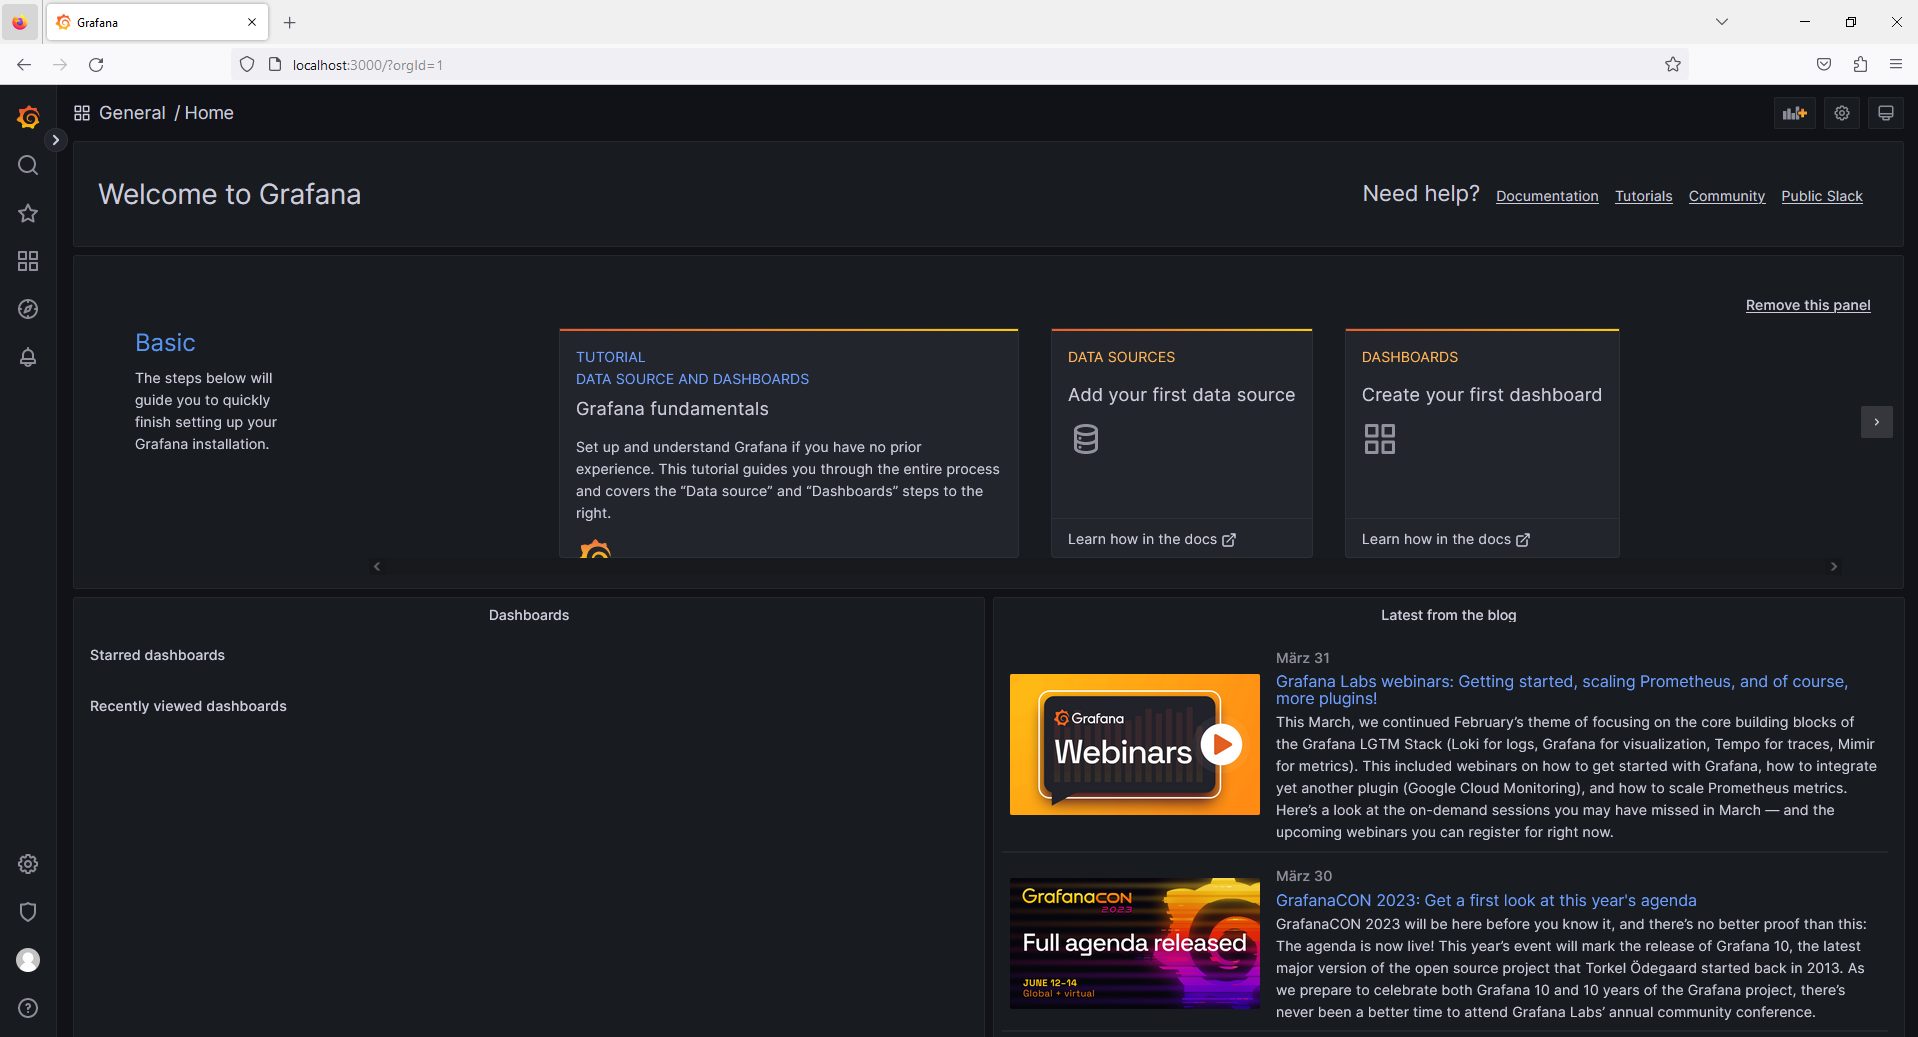
\includegraphics[width=1.3\textwidth]{assets/Installation_Grafana.png}.
         \caption{Screenshot der Willkommensseite von Grafana Loki\\Quelle: Eigene Quelle und \citep{Grafana_Logs}}
         \centering
      \end{figure}
   \end{center}
\end{landscape}

\subsubsection{Weiterleitung der Logdateien zum Grafana}
Grafana Loki bietet einige Möglichkeiten an, um Logdateien weiterzuleiten. In unserer Arbeit benutzen wir \textbf{Promtail}, der in einem \gls{container} läuft. Dieser Instanz schickt Grafana die von uns ausgewählten Logdateien und bearbeitet alle diese Dateien innerhalb eines sogenanntes \quotes{job}. Hätten wir verschiedene Art von Logdateien, würde jeder Typ einem \quotes{job} zugewiesen \citep{Grafana_CollectLogs}. Jeder \quotes{job} hätte ihre eigene Regeln, um nach dem gewünschten Information zu suchen. 

In einen produktive Umgebung wäre die Installation von \textbf{Grafana Agents} in jedenm\gls{Endpoint} eine andere Lösung, um Grafana Loki  Logdateien zu schicken. In diesem Fall würde jeder \gls{Endpoint} 
mithilfe von Promtail die Dateien weiterleiten \citep{Grafana_Agents}. Wie in unserer Lösung, müsste der Nutzer für jeden Art von Logdateien einen spezifischen \quotes{job} konfigurieren. 

Inhalt von Logdateien lassen sich auch mit \textbf{\glsfirst{API}} zum Grafana Loki schicken. In dieser Situation schickt der \gls{Endpoint} einen \gls{http} POST request zum Grafana Loki \gls{Endpoint} mit den Inhalt der Logdateien \citep{Grafana_api}:

{\setstretch{1.0}
\begin{Verbatim}[frame=single]
# Endpoint
POST /loki/api/v1/push

# Inhalt
{
  "streams": [
    {
      "stream": {
        "label": "value"
      },
      "values": [
          [ "Zeit in Unixformat", "<Inhalt der Logdateie>" ],
      ]
    }
  ]
}
}



Die Logdateien lassen sich mithilfe von Grafana Agent zum Grafana weiterleiten. Die Agents werden in jeden Endpoint installiert


\textcolor{red}{\textbf{Erklären über existierenden Möglichkeiten Logdateien weiterzuleiten}}

\subsection{Aufbau der Erkennungsregel für den ausgewählten Angriff}
Der \gls{bruteforce} lässt sich durch die Anzahl des fehlgeschlagen Anmeldungsversuchs erkennen \citep{Selvaganesh_SplunkBruteForce}. Wir bearbeiten eine Situation, in der es keine Gegenmaßnahmen, wie Kontosperre nach \textit{n} beliebigen Versuchen oder \gls{mfa}, implementiert sind. Das folgende Aktivitätsdiagramm stellt einen allgemeinen Ablauf eines Anmeldungsverfahrens dar:

\begin{figure}[H]
   \centering
   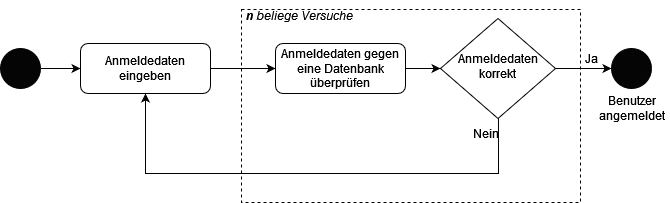
\includegraphics[width=0.8\textwidth]{assets/Anmeldeverfahren.drawio.png}
   \caption{Allgemeiner Ablauf eines Anmeldungsverfahrens \\Quelle: Eigene Quelle und \citep{Selvaganesh_SplunkBruteForce}}
   \centering
\end{figure}

Eine Erkennungsregel hätte folgende Logik:
{\setstretch{1.0}
\begin{Verbatim}[frame=single]
   # Gefundenen Wert in den Logdateien
   # Av = Anzahl fehlgeschlagenen Anmeldungsversuche
   # Ia = Intervallzeit zwischen fehlgeschlagenen Anmeldungsversuche

   # Festgestellte Werte für legitime und bösartige Verbindungen
   # Ga = Grenze zwischen legitimen und bösartigen Anmeldungsversuchen
   # Nt = Intervallzeit zwischer legitime Anmeldungsversuche

   wenn (Av >= Ga) und (Ia < Nt)
      Warnmeldung(Brutefoce)
   sonst
      weiterBeobachten()
\end{Verbatim}
}

\newpage
Grafana Loki bietet einen Einstellungsmuster für die Eingabe und Darstellung von \gls{ssh} Logdateien an. In dieser Einstellung befinden sich schon Graphik und Regelsätze für eine umfangreiche Analyse dieser Daten \citep{VoidQuark_sshlogs}. Die extrahierte Logdateien werden mit folgenden Elementen gelesen und bearbeitet:

\begin{table}[H]
   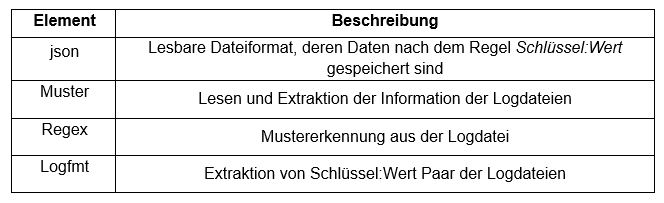
\includegraphics[width=\linewidth]{assets/tabelle_sshgrafana.png}
   \caption{Aufbau der Regelsätze in Grafana Loki für \gls{ssh} Logdateien \\Quelle: Eigene Quelle, \citep{VoidQuark_sshlogs} und \citep{Setter_Logfmt}}
\end{table}

Jedes Angriffszenario hat spezifische Regeln, die mit \gls{logql}  aufgebaut sind. In Promtail wird jeder \gls{Endpoint} \quotes{Instance} genannt. Eine oder mehrere \quotes{Instance} werden einem \quotes{Job} zugewiesen. Diese Struktur kommt aus dem Tool \gls{prometheus}. Die \quotes{Instances} in einem \quotes{Job} werden nach dem gleichen Regeln bearbeitet. Die Abfrage für unseren Angriff sieht so aus \citep{VoidQuark_sshlogs}:

{\setstretch{1.0}
\begin{Verbatim}[frame=single]
(1) - "sum by (username) (count_over_time({$label_name=~\"$label_value\",
      job=~\"$job\", instance=~\"$instance\"} 
(2) - |=\"sshd[\" 
(3) - |=\": Failed\" !~\"invalid user\" 
(4) - | pattern `<_> for <username> from <_> port` 
(5) - | __error__=\"\" [$__interval]))",

(1) - Aufsummierung der Benutzername, den dieser Regel entsprechen und 
      Filtern nach dem Job und Instance
(2) - Suche nach Zeilen mit dem Wort "sshd"
(3) - Suche nach Zeilen mit dem Wort "Failed" und ohne den Ausdruck 
      "invalid user"
(4) - Extrahierung des Benutzernames und der Port der Zeilen
(5) - Suche nach andere Fehlermeldung, falls vorhanden
\end{Verbatim}
}



\textcolor{red}{\textbf{Hinzufügen wie es in Grafana aufgebaut ist. Abschnitt der Regel und Erklärung}}

\textcolor{red}{\textbf{wie würde es für andere Logs aussehen}}

\newpage
\thispagestyle{lscape}
\begin{landscape}
   Nachdem die \gls{ssh}-Logdateien gelesen und bearbeiten wurden, bekommen wir von Grafana Loki folgende Zasammenfasung der Ergebnissen:
   \begin{center}
      \begin{figure}[H]
         \centering
         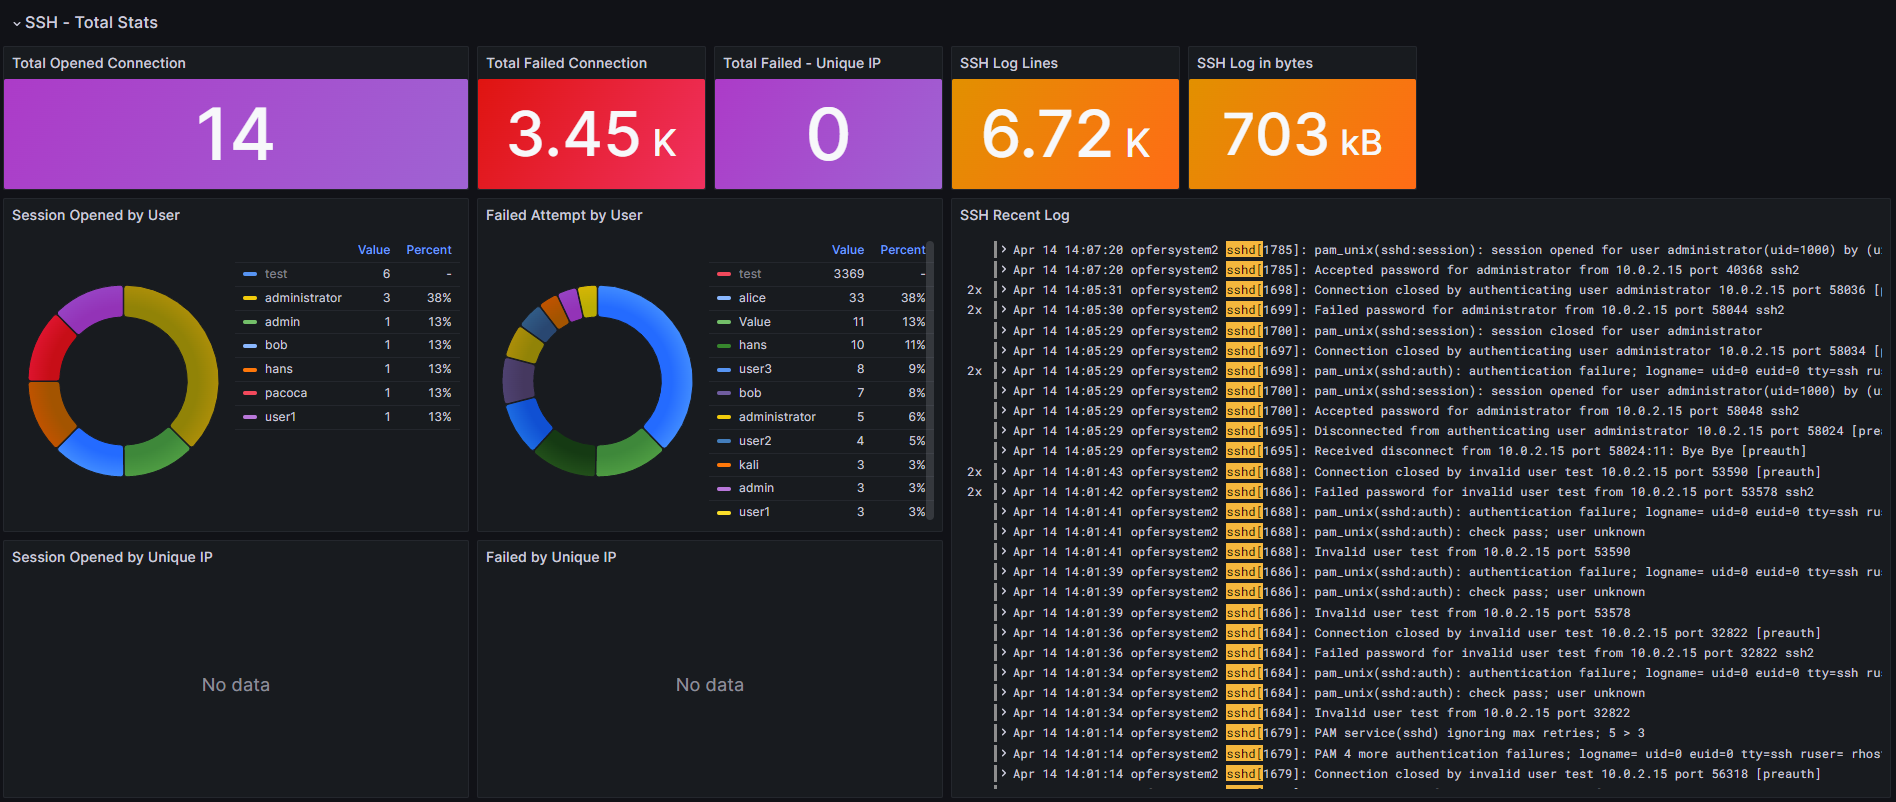
\includegraphics[width=1.3\textwidth]{assets/GrafanaLoki_ssh.png}.
         \caption{Bearbeitung der \gls{ssh} Logdateien von Grafana Loki\\Quelle: Eigene Quelle and \citep{VoidQuark_sshlogs}}
         \centering
      \end{figure}
   \end{center}
\end{landscape}

\newpage
\thispagestyle{lscape}
\begin{landscape}
   Das nächste Bild gibt ausführliche Informationen der Logdateien:
   \begin{center}
      \begin{figure}[H]
         \centering
         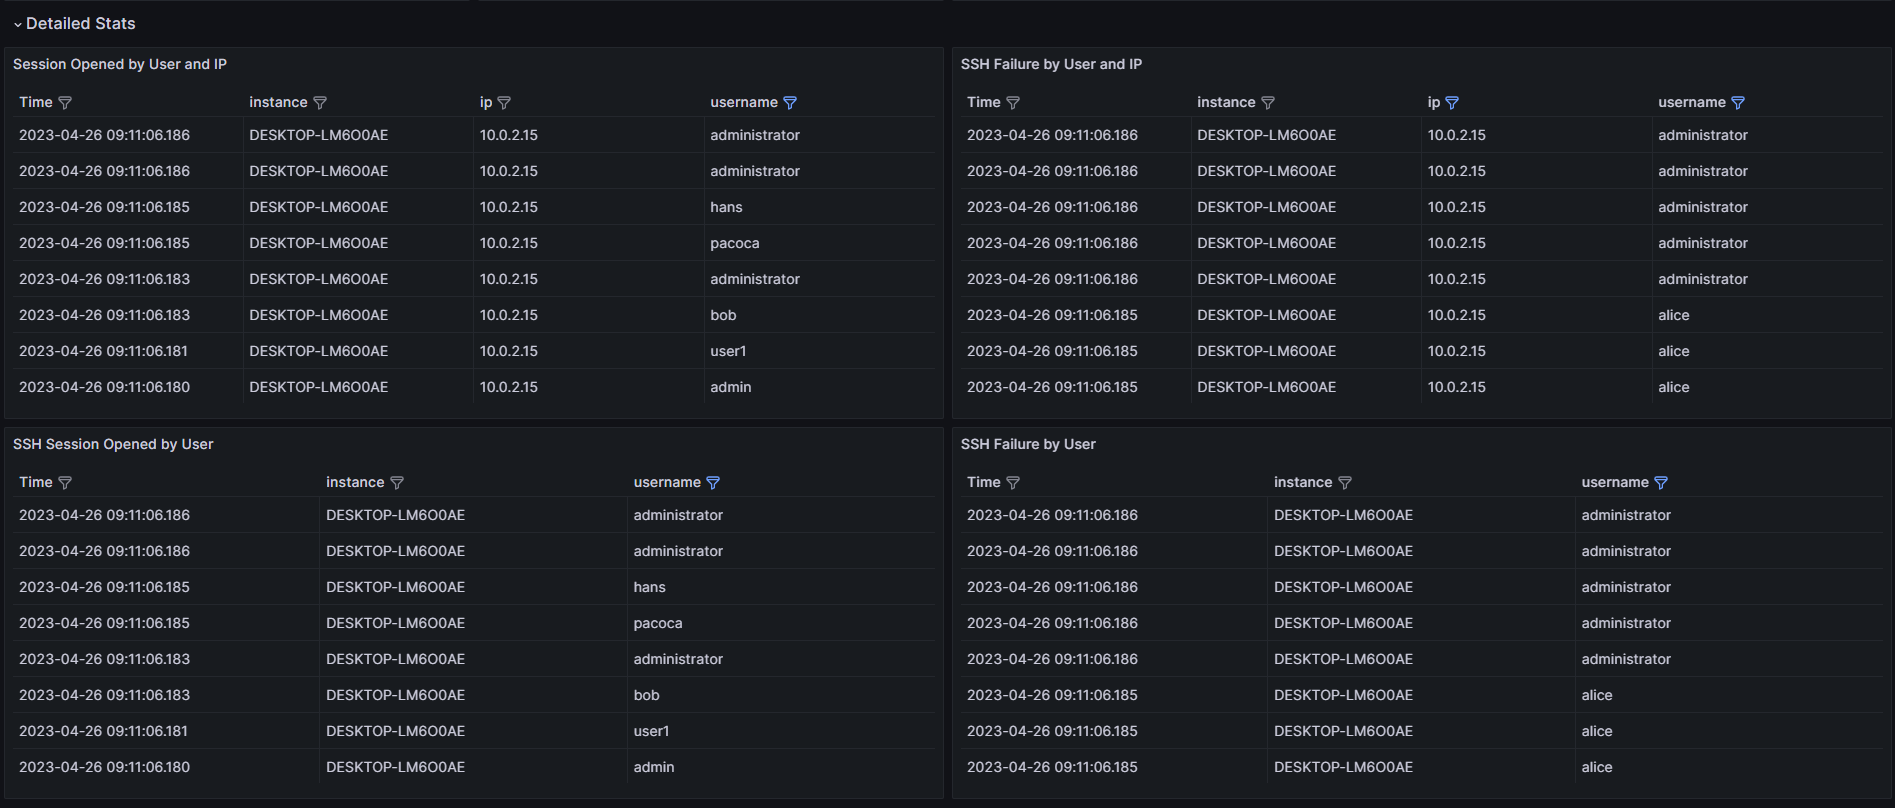
\includegraphics[width=1.3\textwidth]{assets/GrafanaLoki_sshDetailed.png}.
         \caption{Ausführliche Darstellung der \gls{ssh} Logdateien von Grafana Loki\\Quelle: Eigene Quelle and \citep{VoidQuark_sshlogs}}
         \centering
      \end{figure}
   \end{center}
\end{landscape}

\subsection{Einrichtung des Warnmeldungskomponent}
Über Alarmsignal zu schreiben

%\textcolor{red}{\textbf{statische vs dinymische Regel}}



% \subsection{Bewertung der Daten in Grafana}
% Hinzufügen der Logdateien und Erstellung von Regeln zur Erkennung des Angriffes
% Diagramm der Nutzung von Grafana

% \subsection{Normalisierung der Logdateien mit Zeek}
% Diagramm der Nutzung von Grafana und Zeek

% Hier werden die Schritte für die Installation und Sammeln von Daten beschrieben.

% - Implementation in Container %https://rdr-it.com/elk-installation-configuration-un-siem-docker/


% \subsection{Sammlung von Server-Log Dateien}

% \subsection{Normalisierung der Log-Dateien}





